\chapter{低维拓扑模型}
\section{霍尔电导的量子化}
从(\ref{hallInduc})可知霍尔电导的量子化实际是chern number的离散取值。这里我们用具有正方形布里渊区的晶格为例子(周期性边界条件)。Chern number可以写开为
\begin{equation}
\begin{aligned}
C_ 1 &= \frac{1}{2 \pi} \int_{0}^{2 \pi} d k_{x} \int_{0}^{2 \pi} d k_{y}\left[\partial_{k_{x}} \mathbf{A}_{y}\left(k_{x}, k_{y}\right)-\partial_{k_{y}} \mathbf{A}_{x}\left(k_{x}, k_{y}\right)\right]\\
&= \frac{1}{2 \pi} \int_{0}^{2 \pi} dk_{y}\left[\mathbf{A}_{y}\left(2 \pi, k_{y}\right)-\mathbf{A}_{y}\left(0, k_{y}\right)\right] -\frac{1}{2 \pi} \int_{0}^{2 \pi} d k_{x}\left[\mathbf{A}_{x}\left(k_{x}, 2 \pi\right)-\mathbf{A}_{x}\left(k_{x}, 0\right)\right] 
\label{chernAsA}
\end{aligned}
\end{equation}
假设布洛赫波在布里渊区边界两边差一个相位因子$\theta$
\begin{equation}
  \ket{u(k_x, 2 \pi)} = \mbox{exp}[\theta_x(k_x)] \ket{u(k_x, 0)}
\end{equation}
可以把这个关系传递到Berry connection
\begin{equation}
  A_x(k_x, 2 \pi) = - \partial_{k_x} \theta_x(k_x) + A_x(k_x, 0)
\end{equation}
同理,在y方向也有
\begin{equation}
A_{y}\left(2 \pi, k_{y}\right)=-\partial_{k_{y}} \theta_{y}\left(k_{y}\right)+A_{y}\left(0, k_{y}\right)
\end{equation}
代入(\ref{chernAsA})可得chern number
\begin{equation}
  C_1 = \frac{1}{2 \pi} [\theta_y(0) - \theta_y(2 \pi) + \theta_x(2 \pi) + \theta_x(0) ]
\end{equation}
考察一下波函数在布里渊区四个顶点的关系
\begin{equation}
\begin{aligned} e^{i \theta_{x}(0)}|u(0,2 \pi)\rangle &=|u(0,0)\rangle \\ e^{i \theta_{x}(2 \pi)}|u(2 \pi, 2 \pi)\rangle &=|u(2 \pi, 0)\rangle \\ e^{i \theta_{y}(0)}|u(2 \pi, 0)\rangle &=|u(0,0)\rangle \\ e^{i \theta_{y}(2 \pi)}|u(2 \pi, 2 \pi)\rangle &=|u(0,2 \pi)\rangle\end{aligned}
\end{equation}
整合可以得到
\begin{equation}
\ket{u(0,0)}=e^{i\left[\theta_{x}(0)+\theta_{y}(2 \pi)-\theta_{x}(2 \pi)-\theta_{y}(0)\right]}|u(0,0)\rangle
\end{equation}
显然,指数上的相位差只能是$2 \pi$的整数倍。因此chern number是量子化的
\begin{equation}
  C_1 = \nu, \nu = 1, 2, ...
\end{equation}
这就是反常量子霍尔效应的来源。
\section{拓扑相变}
一个模型通常可以采用调节哈密顿量H里的某个参数来实现chern number在平凡(等于$0$)和
非平凡(不等于$0$)之间转化。Chern number的改变又叫做拓扑相变。能实现拓扑相变的
最简单的模型就是具有两个能带的Su-Schrieffer-Heeger模型
 \begin {figure}[tbp]
\centering 
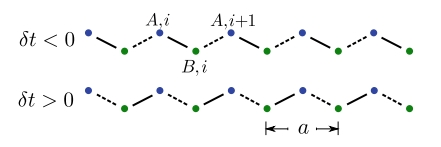
\includegraphics[width=10cm]{./images/sshmodel.jpg} 
\caption{SSH模型。每个原胞内具有AB两种原子。实现表示两个端点具有强度为$t+\delta t$的相互作用,虚线则表示相互作用强度为$t – \delta t$。这个模型具有开边界条件\cite{topoText}}
\label{sshmodel}
\end {figure} 

从紧束缚模型那一节的讨论可以很快写出这个模型的哈密顿量
\begin{equation}
H=\sum_{n=1}^{N}(t+\delta t) c_{A, n}^{\dagger} c_{B, n}+\sum_{n=1}^{N-1}(t-\delta t) c_{A, n+1}^{\dagger} c_{B, n}+h . c
\end{equation}
写成矩阵形式为
\begin{equation}
H=\left(\begin{array}{ccccccc}0 & t+\delta t & 0 & 0 & 0 & 0 & 0 \\ t+\delta t & 0 & t-\delta t & 0 & 0 & 0 & 0 \\ 0 & t-\delta t & 0 & t+\delta t & 0 & 0 & 0 \\ 0 & 0 & t+\delta t & 0 & t-\delta t & 0 & 0 \\ 0 & 0 & 0 & t-\delta t & 0 & \ddots & 0 \\ 0 & 0 & 0 & 0 & \ddots & 0 & t+\delta t \\ 0 & 0 & 0 & 0 & 0 & t+\delta t & 0\end{array}\right)
\end{equation}
这个矩阵比较简单,可以通过数值的方法对角化来求得体系的能带。另一方面,我们也可以
采用紧束缚模型那一节所采用的方法来:把$c_{A, n}$做傅里叶展开。这样得到的$M^{ab}_k$矩阵表达式为
\begin{equation}
  M_k = \left[((t+\delta t)+(t-\delta t) \cos k) \sigma_{x}+(t-\delta t) \sin k \sigma_{y}\right] 
\end{equation}
为了方便计算,我们做一个变换$\sigma_x \rightarrow \sigma_z, \sigma_y
\rightarrow \sigma_x, \sigma_z \rightarrow \sigma_y$, and $k \rightarrow k + \pi$ $M_k$ 被变换为
\begin{equation}
  M_k = -(t - \delta t) \text{sin}k \sigma_x + (2 \delta t + 2 (t - \delta t) \text{sin}^2\frac{k}{2}) \sigma_z
\end{equation}
对角化$M_k$可以得到能带表达式
\begin{equation}
  E_{\pm} = \pm (d_x^2 + d_z^2)
\end{equation}
其中$d_x = -(t - \delta t) \text{sin}k$,$d_x = 2 \delta t + 2 (t - \delta t) \text{sin}^2\frac{k}{2}$, 本征向量可以用来计算下能带的一维的chern number (又叫做winding number),结果为(\cite{topoText})
\begin{equation}
  (-1)^\nu = \text{sgn}(\delta t) \text{sgn}(\delta t + t)
\end{equation}
其中$\nu$是winding number。注意这里的$\delta t$ 应该是远小于$t$的,就是说当$\delta t$小于0时,winding number是1,大于0时winding number是0. 因此我们可以通过改变$\delta t$的符号来实现拓扑相变。考察$k=0$附近的能带随$\delta t$ 的变化可以直观地显示这个过程。把$E(k)$在0处展开,略去高阶小量可以得到
\begin{equation}
  E(k) = \pm \sqrt{(t - \delta t)^2 k^2 + 4 \delta t^2}
\end{equation}
$k = 0$时的能带间隙为$4\delta t$。因此$\delta t$从负数增大到0时,能带间隙变小,在等于0时贴合。而$\delta t$增大为正数后又打开了能隙。尽管变化前后能带的形状相同,但它们已具有不同的winding number,因此具有不同的物理性质,是不同的拓扑相。

\section{Edge Mode}

求解下面这个二维模型可以解释chern number背后的物理
\begin{equation}
\begin{aligned} H= \sum_{k_{y} x}\left\lfloor c_{k_{y}}^{\dagger}(x) \frac{\sigma_{z}-i \sigma_{x}}{2} c_{k_{y}}(x+1)+\text { h.c. }\right]+\sum_{k_{y} x} c_{k_{y}}^{\dagger}(x)\left[\sin k_{y} \sigma_{y}\right. \left.+\left(m+\cos k_{y}\right) \sigma_{z}\right] c_{k_{y}}(x) \end{aligned}
\end{equation}
这个模型是一个柱面。它在y方向上是具有周期性边界条件,在x方向是上则是开边界(图{\ref{edgePPT}。a)。取特定的m值可以使得下能带chern number = 1,上能带为-1,其对应的能带如图{\ref{edgePPT}.b。

每一个特定的$k_y$都有N个本征值。这些本征值来源于x方向上的N个晶格。整个能谱图被划分为对应不同颜色的三个部分。蓝色点代表的本征值来源于材料的内部。换句话说,蓝色本征值对应的波函数在材料内部是一个扩散的状态。而黑色或者红色点的波函数则局域在x方向上的两个边界(波函数在材料内部为0)。因此黑色和红色线被称作是edge mode。

%图:edge mode 的波函数。横坐标i是格点序号。波函数局域在系统的边界。当$\delta$趋向于0,能隙变小,edge mode 被“削弱”,波函数出现往系统内部扩散的现象。
\begin {figure}[tbp]
\centering 
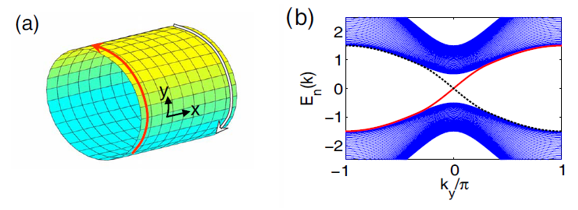
\includegraphics[width=14cm]{./images/edgePPT.png} 
\caption{(a)一个柱面材料。它在y方向上是周期性边界条件,x方向上是开边界。取特定的m参数,会在两个边界产生edge mode(b) 模型的能带图。图中每一个点都是哈密顿量的一个本征值,连起来便形成能带。图被分为上下能带,中间还有红黑两条edge mode}
\label{edgePPT}
\end {figure} 

Edge mode 的存在会产生新奇的物理现象。由半经典方程可以知道,在材料的y方向上通上
均匀电场等价于对$k_y$做一个随时间线性相关的平移 $k_y \rightarrow k_y - E_y t$。从能
谱图上看就是有一条$k_y = k_{y0} – E_y t$的轴线随时间扫描过整个能带图。电子具有从
低能级开始填充能带的性质。假设开始时费米能级恰好在$E = 0$处,即电子填满下能带且
恰好填到图中的$(0, 0)$点,那么当$k_y$走向往左扫描时,电子会沿着红线走,并走到下
能带,然后一直走到$k_y = -\pi$处。由于材料在$k_y$方向是周期的,扫描线会继续从
$k_y= \pi$处往左扫描,并使电子走出下能带,走入黑线,最终走回$(0, 0)$点。总之,这个红线—下能带—黑线的过程会随时间一直循环下去。
  从波函数的角度看上述过程可以理解为什么会在x方向上有电流产生。一开始电子填充的
  是红线,波函数被局域在$x = 0$处边界。之后电子进入下能带,波函数相当于从$x = 0$
  处扩散到材料内部,并在电子填充到黑线时到达$x = L$处边界。波函数是概率,也就是电荷密度,因此x方向上会存在电流,这就是霍尔电流。
  
Edge mode 数量和不同能带的chern number 有如下关系
\begin{equation}
n_{L}\left(E_{g}\right)-n_{R}\left(E_{g}\right)=\sum_{E_{n}<E_{g}} \operatorname{Ch}\left(E_{n}\right)
\end{equation}
其中$\operatorname{Ch}(E_n)$是第$n$个能带的chern number。真空的chern number是$0$.Eg是能隙。$n_L(E_g)$和$n_R(E_g)$是出现在系统左边界的左旋和右旋chiral mode数量。注意一个体系总体上必须是拓扑平庸的,因此所有的能带chern number 和必须为0.在图像上表现为上顶带上方无edge mode。
下面的这个哈密顿量是一个很好的例子
\begin{equation}
H=\sum_{j=1}^{N}\left[-t\left(c_{j}^{\dagger} c_{j+1}+c_{j+1}^{\dagger} c_{j}\right)-V \cos \left(2 \pi \frac{p}{q} j+\theta_{0}\right) c_{j}^{\dagger} c_{j}\right]
\end{equation}
它对应的能谱如图\ref{edgeHe}.
\begin {figure}[tbp]
\centering 
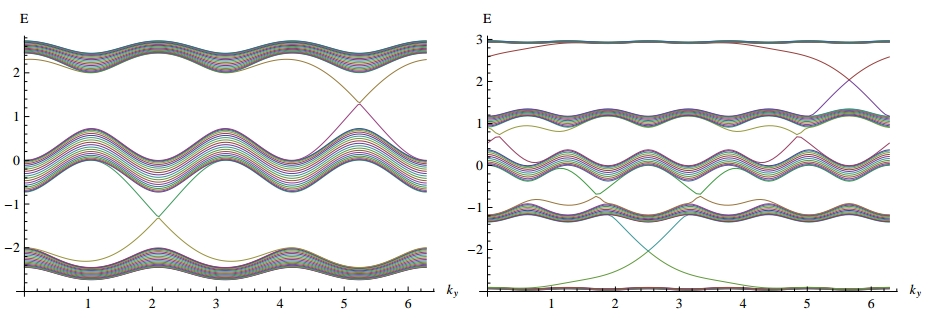
\includegraphics[width=13cm]{./images/edgeHe.jpg} 
\caption{左侧能谱图取数$p/q = 1/3$。从下往上的能带完全充满时chern number分别为1,-2,1. 右侧$p/q=1/5$,chern number分别为1,1,-4,1,1}
\label{edgeHe}
\end {figure} 

右侧子图第一个能隙(从下往上数)下面仅有一条能带,对应的$\operatorname{Ch}(E_0) = 1$, 因此系统左边界仅仅有一个edge mode。图中另一条edge mode是右边界产生的。第二个能隙下面有两个能带,对应chern number和为2,因此有4条edge mode(左右边界各两个)。其它能隙也有类似的推理。